\documentclass[tikz, preview]{standalone}

\usepackage{amsfonts, amsthm, amssymb, amsmath, stmaryrd, etoolbox}
\usepackage{tikz}
\usepackage[all,2cell]{xy}
\usetikzlibrary{matrix,arrows,shapes,decorations.markings,decorations.pathreplacing}
\definecolor{rewritecolor}{rgb}{0,.9,1}
\tikzset{rewritenode/.style={shape=circle,fill=rewritecolor,scale=0.25,font=\Huge}}
\tikzset{RWopen/.style={shape=circle,draw=black,fill=white,scale=0.5,font=\Huge}}
\tikzset{RWclosed/.style={shape=circle,fill=black,scale=0.5,font=\Huge}}
\tikzset{CDnode/.style={shape=circle,fill=white,scale=.5}}
\tikzset{zxgreen/.style={shape=circle,draw,thick,fill=green}}
\tikzset{zxred/.style={shape=circle,draw,thick,fill=red}}
\tikzset{zxyellow/.style={shape=rectangle,draw,thick,fill=yellow}}
\tikzset{zxdiamond/.style={shape=diamond,fill=black,inner sep=2.75}}
\tikzset{zxopen/.style={shape=circle,draw,thick,inner sep=2pt}}
\tikzset{->-/.style={decoration={markings,mark=at position .5 with {\arrow{>}}},postaction={decorate}}}
\tikzset{->-pos/.style={decoration={
			markings,
			mark=at position #1 with {\arrow{>}}},postaction={decorate}}}


\begin{document}
\[
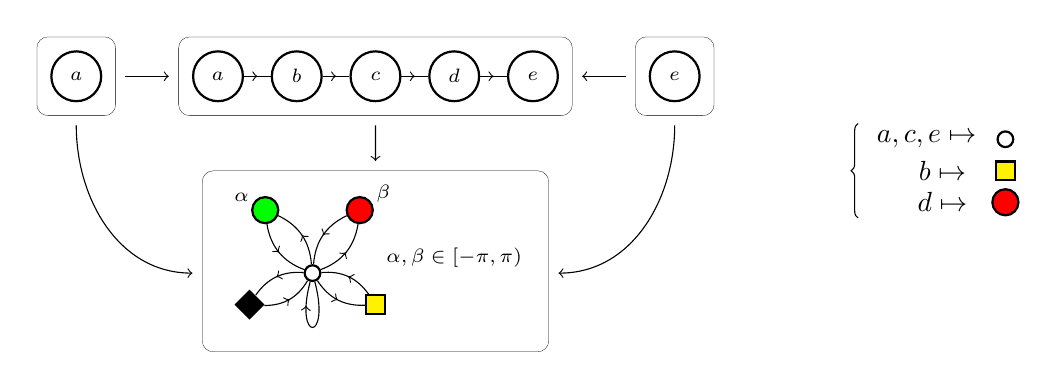
\begin{tikzpicture}
\begin{scope}[shift={(0,0)}]
\node [circle,draw,thick,minimum size=18pt] (a) at (0,0) {\scriptsize $a$};
\node [circle,draw,thick,minimum size=18pt] (b) at (1,0) {\scriptsize $b$};
\node [circle,draw,thick,minimum size=18pt] (c) at (2,0) {\scriptsize $c$};
\node [circle,draw,thick,minimum size=18pt] (d) at (3,0) {\scriptsize $d$};
\node [circle,draw,thick,minimum size=18pt] (e) at (4,0) {\scriptsize $e$};
%
\draw [->-] (a) to (b);
\draw [->-] (b) to (c);
\draw [->-] (c) to (d);
\draw [->-] (d) to (e);
%
\node (um1) at (-0.5,0) {};
\node (um2) at (2,-0.5) {};
\node (um3) at (4.5,0) {};
\node (rect1) at (-0.5,0.5) {};
\node (rect2) at (4.5,-0.5) {};
\draw [ultra thin, rounded corners] (rect1) rectangle (rect2);
\end{scope}
%
%
%
\begin{scope}[shift={(-1.8,0)}]
\node [circle,draw,thick,minimum size=18pt] (a) at (0,0) {\scriptsize $a$};
%
\node (ul1) at (0.5,0) {};
\node (ul2) at (0,-0.5) {};
\node (rect1) at (-0.5,0.5) {};
\node (rect2) at (0.5,-0.5) {};
\draw [ultra thin, rounded corners] (rect1) rectangle (rect2);
\end{scope}
%
%
%
\begin{scope}[shift={(5.8,0)}]
\node [circle,draw,thick,minimum size=18pt] (a) at (0,0) {\scriptsize $e$};
%
\node (ur1) at (-0.5,0) {};
\node (ur2) at (0,-0.5) {};
\node (rect1) at (-0.5,0.5) {};
\node (rect2) at (0.5,-0.5) {};
\draw [ultra thin, rounded corners] (rect1) rectangle (rect2);
\end{scope}
%
%
%
\begin{scope}[shift={(9.2,-0.8)}]
\node at (-0.2,0) {$a,c,e \mapsto$};
\node at (0,-0.4) {$b \mapsto$};
\node at (0,-0.8) {$d \mapsto$};
\node [zxyellow] at (0.8,-0.4) {};
\node [zxred] at (0.8,-0.8) {};
\node [zxopen] at (0.8,0) {};
\node (1) at (-1,0.2) {};
\node (2) at (-1,-1) {};
\draw [decoration={brace,mirror,raise=2pt},decorate] (1.center) -- (2.center); 	
\end{scope}
%
%
%
\begin{scope}[shift={(1.2,-2.8)}]
\node [zxopen] (v1) at (0,0.3) {};
\node [zxgreen,label={[shift={(-.3,-.2)}]\scriptsize $\alpha$}] (v2) at (-0.6,1.1) {};
\node [zxyellow] (v3) at (0.8,-0.1) {};
\node [zxdiamond] (v5) at (-0.8,-0.1) {};
\node [zxred,label={[shift={(.3,-.2)}]\scriptsize $\beta$}] (v4) at (0.6,1.1) {};
\node at (1.8,0.5) {\scriptsize $\alpha, \beta \in [-\pi,\pi)$};
%
\draw [->-] (v1) to [bend right] (v2);
\draw [->-] (v2) to [bend right] (v1);
\draw [->-] (v1) to [bend right] (v3);
\draw [->-] (v3) to [bend right] (v1);
\draw [->-] (v1) to [bend right] (v4);
\draw [->-] (v4) to [bend right] (v1);
\draw [->-] (v1) to [bend right] (v5);
\draw [->-] (v5) to [bend right] (v1);
\draw [->-pos=0.75] (v1) to [loop below, looseness=35] (v1);
%
\node (l1) at (-1.4,0.3) {};
\node (l2) at (0.8,1.6) {};
\node (l3) at (3,0.3) {};
\node (rect1) at (-1.4,1.6) {};
\node (rect2) at (3,-0.7) {};
\draw [ultra thin,rounded corners] (rect1) rectangle (rect2);
\end{scope}
%
%
%
\draw [->] (ul2) edge [out=-90,in=-180] (l1);
\draw [->] (ul1) edge [] (um1);
\draw [->] (um2) edge [] (l2);
\draw [->] (ur1) edge [] (um3);
\draw [->] (ur2) edge [out=-90,in=0] (l3);
\end{tikzpicture}
\]
\end{document}
